\section{Using SCA Tools in White-Box Cryptography}
\label{sec:scawbc}

In the previous section we presented some algorithms seemingly unrelated to what we have done so far. Indeed, our aim is to attack white-box implementations where we can fully control the execution environment thus there is no need for physical measurements. The actual reason emerges from a groundbreaking approach introduced recently by Bos et al.\ \cite{bos2015differential} -- the use of SCA tools in white-box cryptography context.

The idea was inspired by Delerabl{\'e}e et al.\ \cite{delerablee2013white}. As it is usually required, a ``perfect'' white-box implementation should not provide effectively any other information about the secret key but only as much as an access to a black-box. In \cite{delerablee2013white} they observed that such implementation must be resistant to all existing and future side-channel attacks which led Bos et al. to the idea of exploring this consequence by attacking white-box implementations with SCA tools. And the attack very surprisingly succeeded!

The obvious question is what kind of traces we should use instead of power traces -- we use {\em software traces}. In this context, software trace reffers to a record of memory addresses being accessed during program execution or their contents, sometimes also referred to as {\em memory trace}. Hence in this context differential power analysis might sound wierd since there is no {\em power}, it is rather referred to as {\em Differential Computation Analysis} (DCA).


% ==============================================================================
% ===   T R A C E   A C Q U I S I T I O N                                    ===
% ==============================================================================

\subsection{Trace Acquisition}
\label{sec:tracq}

In order to acquire a memory trace we use Dynamic Binary Instrumentation (DBI) tools. These tools insert additional instructions to the original code of the program at run-time enabling one to debug or detect memory leaks. The most advanced DBI tools like Valgrind \cite{nethercote2007valgrind} or PIN \cite{luk2005pin} include a programmable interface where you can write tools of your will. Both tools are open-source.

We modified a tool for PIN by Teuwen \cite{teuwen2015movfuscator} for $4$ use cases. These acquire
\begin{enumerate}
	\item addresses of memory reads, \label{item:readaddr}
	\item addresses of memory writes,   %!% neni
	\item contents of memory reads, and   %!% neni
	\item contents of memory writes, \label{item:writecnt}
\end{enumerate}
respectively. Tool nr.\ \ref{item:writecnt} is obviously most useful for unprotected implementations since it can directly observe byproducts, tool nr.\ \ref{item:readaddr} will be surprisingly used as well. The other tools will not be used.

\begin{note}
\label{note:lsb}
	So far we have not specified any possible limitations on memory traces. Note that in case we are catching addresses, we can limit our attention to the least significant byte only. Indeed, the rest of the address does not contain any relevant information, only the global position in memory. On the other hand, the least significant byte carries information about the position within an array representing a WBAES table.
	
	In case of reading memory contents, we can only be interested in $1$ byte memory reads/writes since AES tables are constructed based on byte-wise representation.
\end{note}

Using chosen tool we acquire certain amount of memory traces with different, possibly random, plaintexts on input. We save these plaintexts along corresponding traces, of course.

\begin{note}
\label{note:optim}
	In order to attack by SCA tools, traces must be properly aligned. It could happen that compiling C/C++ programs with high levels of optimization would produce misaligned traces; we actually experienced different lengths of traces.
	
	Therefore we recommend to compile C/C++ programs with different levels of optimization and acquire just a few traces for each level. We check traces' lengths and apply the highest optimization level where the traces were equally long and use this optimization level for trace acquisition.
\end{note}

One may wonder whether traces can ever be properly aligned at all because then it would require additional effort to align them. According to our experience, traces are well aligned hence there should be no need for this.

\begin{note}
\label{note:aslr}
	There is another issue with trace acquisition, now it is related to the next step which is trace filtering. It will be appreciated if the program uses very the same addresses for instructions which are not plaintext related. Later we will try to filter them out since they do not carry any useful information.
	
	For this reason it might be helpful to switch off Address Space Layout Randomization (ASLR) and acquire all traces in a single terminal session.
\end{note}

Having traces properly acquired, let us proceed to trace filtering.


% ==============================================================================
% ===   T R A C E   F I L T E R I N G                                        ===
% ==============================================================================

\subsection{Trace Filtering}
\label{sec:filter}

Once we have acquired memory traces, we perform two kinds of filtering. We filter trace entries
\begin{itemize}
	\item by constant value, and
	\item by address and temporal range.
\end{itemize}

\subsubsection{Constant Entries Filtering}
	
	In the first stage we filter out such entries which are constant across all acquired traces because they do not carry any information. Indeed, both presented SCA algorithms exploit changes across traces.
	
	Practically we first create a filter mask based on a small set of traces, $10$ shows to be sufficient. Such mask carries $0$ if all corresponding addresses in the small set of traces are equal, $1$ otherwise, see Figure \ref{fig:constmask}. This mask is then simply applied to filter all the remaining traces, possibly hundreds or thousands of them. Note that we keep the mask, we will use it for the following filtering method as well.
	
	\begin{figure}[H]
	\[
	\arraycolsep=.5em\def\arraystretch{1.5}
		\begin{array}{|c|ccccccccc|}
			\hline
			\textnormal{Trace 0} & {\tt 65} & {\tt de} & {\tt 37} & {\tt 7e} & {\tt 63} & {\tt 30} & {\tt c0} & {\tt 62} & {\tt 61} \\
			\textnormal{Trace 1} & {\tt 65} & {\tt de} & {\tt 31} & {\tt 7e} & {\tt 23} & {\tt 30} & {\tt b1} & {\tt 62} & {\tt 61} \\
			\textnormal{Trace 2} & {\tt 65} & {\tt de} & {\tt 1f} & {\tt 7e} & {\tt d5} & {\tt 30} & {\tt 77} & {\tt 62} & {\tt 61} \\
			\textnormal{Trace 3} & {\tt 65} & {\tt de} & {\tt 97} & {\tt 7e} & {\tt 5c} & {\tt 30} & {\tt c4} & {\tt 62} & {\tt 61} \\
			\hline
			\textnormal{Mask}    & {\tt 0}  & {\tt 0}  & {\tt 1}  & {\tt 0}  & {\tt 1}  & {\tt 0}  & {\tt 1}  & {\tt 0}  & {\tt 0} \\
			\hline
		\end{array}
	\]
	\caption{An example of a mask used for trace filtering.}
	\label{fig:constmask}
	\end{figure}
	
	\begin{note}
	\label{note:filter}
		Filtering of constant entries typically decreases the size of the traces by tens of percent. If you do not observe any or extremely small decrease, it might have happened that the traces are not properly aligned. In such case it might be very difficult to align them. Luckily we did not experience this problem and give some advices how to avoid it in Note \ref{note:aslr}.
	\end{note}

\subsubsection{Address and Temporal Filtering}
	
	In the second stage we will filter the traces based on visual observation. Note that for this purpose we will need to acquire another trace with full read/write addresses for all memory trace types, unlike Note \ref{note:lsb}. We will refer to such trace as {\em full trace}.
	
	We will proceed as follows: first we acquire a full trace and filter it by the mask from the previous method. Then we visualize it and try to find out in which address and temporal range encryption takes place. Based on our observation we filter our traces using this range.
	
	\begin{note}
	\label{note:fullfilter}
		Once we filter the full trace, we get rid of tons of ballast yielding a trace which is much smaller and easier to understand. Note that the filtered full trace is also correctly aligned to the rest of our traces after filtering.
	\end{note}
	
	\paragraph{Trace Visualization}
		
		We developed own tool displaying a full memory trace for this purpose. Given $n$ and a trace, this tool splits the trace by addresses into $n$ ``compact'' segments and displays these parts separately. See Figure \ref{fig:memtrace} for an illustrative memory trace of a run of a simple AES implementation. Horizontal axis represents address range, vertical axis represents the order of addresses from the top (temporal range).
		
		\begin{figure}[h!] %!% opravit nakonec
		\begin{center}
			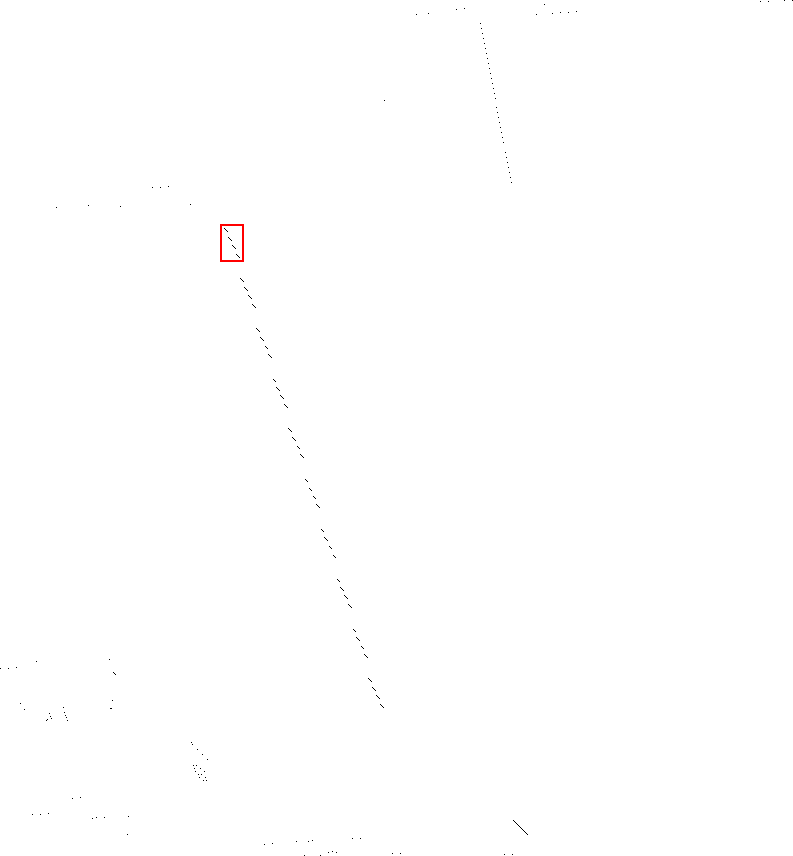
\includegraphics[width=0.9\textwidth]{./figures/memtrace/memtrace_emph.png}
			\caption{Illustrative memory trace of a run of an AES implementation with the first round emphasized by a red rectangle. Addresses of memory writes were acquired.}
			\label{fig:memtrace}
		\end{center}
		\end{figure}
		
		In this example trace we can clearly recoginze $10$ distinct AES rounds even with its $4$ subroutines. In general, if possible, we try to estimate the address and temporal range of the first round\footnote{Note that we are only interested in the first round, see Equation \ref{eq:byprod} and its context.} based on visual observation. In our example the first round is emphasized by a red rectangle.

	\paragraph{Trace Filtering}
		
		Given an address and temporal range, we filter our traces so that we only keep their entries which fall into this range. But our traces do not contain full address information, see Note \ref{note:lsb}. The idea could be to use full traces instead.
		
		If we had all full traces, we could filter them easily based on both ranges. But in this case there may occur a position for which some traces contain an address falling inside or outside the address range, respectively. Note that this would immediately violate the alignment!
		
		\begin{remark}
		\label{rem:rangemask}
			There is a better way how to filter our traces by address and temporal range. We simply take our single filtered full trace and create another mask, see Example \ref{ex:rangemask}. Then we filter our traces with this mask as we did before. This approach ensures that the traces keep aligned.
		\end{remark}
		
		\begin{example}
		\label{ex:rangemask}
			Let say we have deduced from trace visualization that the first round of AES encryption takes place between rows $0$ and $2$ and in an address range from {\tt 0x7fffe3150000} to {\tt 0x7fffe3158000}. Then we get the mask as follows.
			\[
			\arraycolsep=.5em\def\arraystretch{1.5}
				\begin{array}{|c|c|c|}
					\hline
					\textnormal{Row} & \textnormal{Filtered Full Trace} & \textnormal{Mask} \\
					\hline
					0 & {\tt 0x7fffe314f028} & {\tt 0} \\
					1 & {\tt 0x7fffe3150ac8} & {\tt 1} \\
					2 & {\tt 0x7fffe3151dc8} & {\tt 1} \\
					3 & {\tt 0x7fffe3152d18} & {\tt 0} \\
					4 & {\tt 0x7fffe3153948} & {\tt 0} \\
					\hline
				\end{array}
			\]
		\end{example}
		
		Note that address and temporal filtering brings the most substantial speedup of the whole attack since its speed depends heavily on the size of the traces. On the other hand, it may happen that we filter our traces too much and loose valuable information i.e.\ the attack does not succeed. In such case we broaden the address and/or temporal range and try again.
		
		Also note that there may occur several $10$-part patterns resembling $10$ AES rounds. Then we need to keep trying them all until we succeed with our attack.
		
		In the worst case, all our filtering attempts fail or we just cannot see any relevant pattern in the memory trace visualization. Then we omit address and temporal filtering at all and attack for instance only the first byte while, hopefuly, obtaining the position where the key leaks i.e.\ where encryption takes place; here we employ the improved output of our SCA algorithm introduced in Note \ref{note:leakpos}. We can look at this position in the visualization and guess some reasonable address and temporal range, use it for filtering and finally attack all $16$ bytes with much smaller traces.


% ==============================================================================
% ===   A T T A C K I N G   T R A C E S                                      ===
% ==============================================================================

\subsection{Attacking Traces}
\label{sec:attack}

Once the traces are acquired, possibly filtered and, most importantly, properly aligned -- it can be deduced from Note \ref{note:filter} and achieved with ideas from Note \ref{note:aslr} --, we can perform the attack. We can use both SCA algorithms presented in this thesis, i.e.\ Algorithm \ref{alg:cpa} or \ref{alg:bitwisedpa}, or any other SCA algorithm of our choice.

\begin{remark}
\label{rem:traceformat}
	Remind that each of our two SCA algorithms was originally designed for a different kind of traces.
	
	In Algorithm \ref{alg:cpa} the traces were supposed to carry information about Hamming weight of byproducts therefore the original attack must be modified to compute Hamming weights of traces' entries. It might not make much sense to compute Hamming weight of both byproduct and trace entries and then their correlation, but this algorithm serves rather as a proof-of-concept. On the other hand it could possibly bring some surprising results so we employed it as well.
	
	In Algorithm \ref{alg:bitwisedpa} the traces were supposed to be a serialization of eight separate traces which should carry only bits of information, see Note \ref{note:concattraces}. Therefore it is crucial in this attack to consider entries of traces as separate bits, not bytes, i.e.\ {\tt [1,0,0,0,0,1,0,0, 0,1,1,0,1,1,0,0]} rather than {\tt [84, 6c]}.
\end{remark}

As outlined in the previous Remark, since now we will consider Algorithm \ref{alg:bitwisedpa} by default unless stated otherwise.

\subsubsection{Processing Results}
	
	As already stated in Note \ref{note:fulllist}, the best key candidate we obtain from a SCA algorithm does not need to be necessarily the correct one, especially when we use it for attacking white-box implementations where there is absolutely no interpretation of what we ``measure'' and no reasoning why it should work at all.
	
	In that note we suggested to output the full list of key candidates together with their ``value'' for each key byte. The original purpose of this was to have some rating of key candidates and then loop through them according to their order and value. In physical world scenario this would likely recover the key in a relatively short time since we assume certain bias in our measurements caused by execution of the cipher.
	% \footnote{Each SCA algorithm may use different meter to compare key candidates, in Algorithm \ref{alg:cpa} it was correlation, in Algorithm \ref{alg:bitwisedpa} it was difference of means.}
	
	But it turns out that looping would be useless in the white-box scenario. Indeed, by empirical observation, the true key byte is typically
	\begin{itemize}
		\item either on the top separated by a gap from the second candidate, or
		\item somewhere in between while the first candidate is separated by a smaller gap,
	\end{itemize}
	see the following example with real data. This observation is especially useful for our $8$ separate lists, see Note \ref{note:eightlists}.
	
	\begin{example}
	\label{ex:gap}
	See the following table for partial results of a real experiment, further comments below.
	%!% spíš to pak vzít odněkud odspod ty data, třeba z 256 trací
		\begin{table}[H]
			\begin{center}
			\begin{tabular}{| c | c | c | c | c | c | c | c | c |}
				\hline
				\multirow{2}{*}{Rank} & \multicolumn{2}{c|}{\nth{4} bit} & \multicolumn{2}{c|}{\nth{5} bit} & \multicolumn{2}{c|}{\nth{7} bit} & \multicolumn{2}{c|}{\nth{8} bit} \\
				\cline{2-9}
					~ & Value & Cand.   & Value & Cand.   & Value & Cand.   & Value & Cand.  \\
				\hline
					1      & 0.3477 & {\tt >15<} & 0.3970 & {\tt 09}   & 0.3374 & {\tt 9d}   & 0.3730 & {\tt 6f}   \\
					2      & 0.3147 & {\tt b5}   & 0.3884 & {\tt d1}   & 0.3196 & {\tt f5}   & 0.3521 & {\tt 8b}   \\
					3      & 0.3110 & {\tt e7}   & 0.3699 & {\tt 65}   & 0.3183 & {\tt 37}   & 0.3451 & {\tt 7b}   \\
					\vdots & \vdots & \vdots     & \vdots & \vdots     & \vdots & \vdots     & \vdots & \vdots     \\
					22     & \vdots & \vdots     & \vdots & \vdots     & 0.2895 & {\tt fc}   & \vdots & \vdots     \\
					23     & \vdots & \vdots     & \vdots & \vdots     & 0.2892 & {\tt >15<} & \vdots & \vdots     \\
					24     & \vdots & \vdots     & \vdots & \vdots     & 0.2890 & {\tt df}   & \vdots & \vdots     \\
					\vdots & \vdots & \vdots     & \vdots & \vdots     & \vdots & \vdots     & \vdots & \vdots     \\
					40     & \vdots & \vdots     & \vdots & \vdots     & \vdots & \vdots     & 0.2840 & {\tt c1}   \\
					41     & \vdots & \vdots     & \vdots & \vdots     & \vdots & \vdots     & 0.2838 & {\tt >15<} \\
					42     & \vdots & \vdots     & \vdots & \vdots     & \vdots & \vdots     & 0.2825 & {\tt b8}   \\
					43     & \vdots & \vdots     & 0.2760 & {\tt be}   & \vdots & \vdots     & \vdots & \vdots     \\
					44     & \vdots & \vdots     & 0.2760 & {\tt >15<} & \vdots & \vdots     & \vdots & \vdots     \\
					45     & \vdots & \vdots     & 0.2759 & {\tt c4}   & \vdots & \vdots     & \vdots & \vdots     \\
					\vdots & \vdots & \vdots     & \vdots & \vdots     & \vdots & \vdots     & \vdots & \vdots     \\
				\hline
			\end{tabular}
			\end{center}
		\caption{Partial results of a real experiment. The true key byte is {\tt 15} and is emphasized with angle brackets.}
		\label{tab:gap}
		\end{table}
		According to the original criterion (i.e.\ picking the candidate with the highest value) we would get {\tt 09} in the \nth{5} bit column, but it is not the correct one -- in this experiment, the true candidate does not have the highest value.
		
		On the other hand, if we consider the gap and modify our criterion to take it into account, we can still get the correct candidate.
	\end{example}
	
	\begin{remark}
	\label{rem:gap}
		According to the observation in the previous example, we can modify our criterion as follows: we choose the candidate which is on the top of any list and has the biggest gap to the second candidate. Note that we can use various methods how to evaluate this gap, e.g. absolute or relative differences of values, and we may obtain different results.
		
		We can further improve this rule by combining gaps\footnote{Depends how we evaluated the gap, e.g. we use summing.} of the same candidate (only when it is on the top). On the other hand, note that if the correct candidate is not on the top of any list, improving this rule does not help either.
		
		Similarly to the idea of Note \ref{note:fulllist}, we can create a list of maximum $8$ candidates (one candidate from each of $8$ lists, see Note \ref{note:eightlists}) and loop through them if the key was not revealed.
	\end{remark}
	
	Applying the rule from the previous remark to the previous example, we find the maximal gap for the \nth{4} target bit, its absolute value is $0.0330$ compared to $0.0086$, $0.0178$ and $0.0209$, its relative value is $9.5\%$ compared to $2.2\%$, $5.3\%$ and $5.6\%$. Hence the best candidate with this rule is {\tt 15} which is the correct one.
	